\documentclass[11pt]{article}
\usepackage[scaled=0.92]{helvet}
\usepackage{geometry}
\geometry{letterpaper,tmargin=1in,bmargin=1in,lmargin=1in,rmargin=1in}
\usepackage[parfill]{parskip} % Activate to begin paragraphs with an empty line rather than an indent %\usepackage{graphicx}
\usepackage{amsmath,amssymb, mathrsfs, dsfont}
\usepackage{tabularx}
\usepackage[font=footnotesize,labelfont=bf]{caption}
\usepackage{graphicx}
\usepackage{xcolor}
%\usepackage[linkbordercolor ={1 1 1} ]{hyperref}
%\usepackage[sf]{titlesec}
\usepackage{natbib}
\usepackage{../../Tianpei_Report}

%\usepackage{appendix}
%\usepackage{algorithm}
%\usepackage{algorithmic}

%\renewcommand{\algorithmicrequire}{\textbf{Input:}}
%\renewcommand{\algorithmicensure}{\textbf{Output:}}



\begin{document}
\title{Lecture 4.5: Parallel transport and the geodesic: more understandings}
\author{ Tianpei Xie}
\date{ Jun. 13th., 2015 }
\maketitle
\tableofcontents
\newpage
\section{More understanding of parallel transport, covariant derivative and affine connection}
\begin{enumerate}
\item The notion of parallel transport or affine connection supplies a way of \emph{moving the local geometry} of a manifold \emph{along a curve}, or, \emph{connecting the tangent space of the nearby points}.

 Note that it is not well-defined to compare the tangent vector at one point with the tangent vector at another point. The parallel transport provides a way to define their relationship via affine transformation.

\item The notion of \emph{covariant derivative} and \emph{affine connection} are equivalent on the Riemannian manifold, whereas the covariant derivative is the \emph{infinitesimal parallel transport}. 

\item These concepts concern the rate of the change of a vector field $\mb{w}$ along a tangent direction $\mb{v} = \dot{\alpha}$ of a parameterized curve. Thus being denoted as $\nabla_{\mb{v}}\paren{\mb{w}}$. \\[5pt]

\item Intuition behind the affine connection:  note that the tangent plane is \emph{rolled} on $\cS$ without slipping or twisting, the point of contact traces out a curve on $\cS$. Conversely, given a curve on $\cS$, the tangent plane can be rolled along that curve. 

This provides a way to identify the tangent planes at different points along the curve: in particular, a tangent vector in the tangent space at \emph{one point} on the curve is identified with a unique tangent vector \emph{at any other point} on the curve. These identifications are always given by \emph{affine transformations} from \emph{one tangent plane to another}.

This notion of \emph{parallel transport} of tangent vectors, by affine transformations, along a curve has a characteristic feature: the point of contact of the tangent plane with the surface always moves with the curve under \emph{parallel translation} (i.e., as the tangent plane is rolled along the surface, the \emph{point of contact} moves). When the point of contact is viewed as the \emph{origin} in the tangent plane (which is then a vector space), and the \emph{movement of the origin} is \emph{corrected by a translation}, so that parallel transport is \emph{linear}, rather than affine.
\begin{figure}[htb]
\centering
\begin{minipage}{0.6\linewidth}
 \centerline{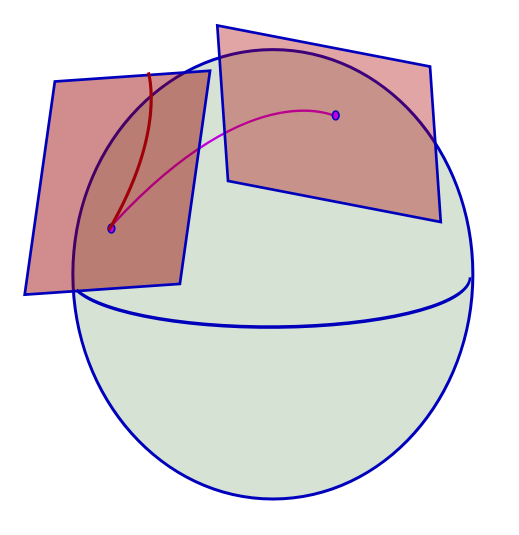
\includegraphics[scale = 0.32]{Parallel_transport_sphere.png}}
\end{minipage}
\caption{\scriptsize
\textbf{The geometric intuition behind the parallel transport along a curve: given a curve on the sphere, the tangent plane can be rolled on the curve without slipping or twisting.  Thus all the tangent plane on the curve can be identified via the affine transformation. }}\label{fig: parallel_transport_sphere}
\end{figure} \vspace{5pt}

\item Motivation of covariant derivative: In differentiating the vector field, the derivatives in component-wise manner do not transform in a manageable way under \emph{changes of coordinates}. In correcting this transformation, additional terms (i.e. the Christoffel symbols) are introduced so that the (corrected) derivative of one vector field along another transformed \emph{covariantly} under coordinate transformations. \\[10pt]

\item In surface in $\bR^{3}$, it is an \emph{affine connection}, satisfies the following properties: for $\mb{w}, \mb{v}, \mb{y}, \mb{z}$ the vector field in $U\subset \cS$ and $f: U \rightarrow \bR$ is a differentiable function in $\cS$; $\mb{y}\paren{f}$ is the directional derivative of $f$ in the direction of $\mb{y}$ (i.e. the direction derivative along the trajectory of vector field $\mb{y}$), $\lambda, \mu$ are real numbers, 
\begin{enumerate}
\item The affine property for vector field 
 \begin{align*}
\nabla_{\mb{y}}\paren{\lambda\mb{w}+ \mu\mb{v}} &= \lambda\nabla_{\mb{y}}\paren{\mb{w}}+ \mu\nabla_{\mb{y}}\paren{\mb{v}}; \\
\nabla_{\lambda\mb{y}+ \mu\mb{z}}\paren{\mb{w}} &= \lambda\nabla_{\mb{y}}\paren{\mb{w}}+ \mu\nabla_{\mb{z}}\paren{\mb{w}}
\end{align*}
\item The Leibniz rule
 \begin{align*}
\nabla_{\mb{y}}\paren{f\mb{w}} &= \mb{y}\paren{f}\mb{w}+ f\nabla_{\mb{y}}\paren{\mb{w}};\\
 \nabla_{f\mb{y}}\paren{\mb{v}} &=  f\nabla_{\mb{y}}\paren{\mb{v}};
\end{align*}
\item The metric-preserving property
\begin{align*}
\mb{y}\paren{\inn{\mb{w}}{\mb{v}}} &= \inn{\nabla_{\mb{y}}\paren{\mb{w}}}{\mb{v}} + \inn{\mb{w}}{\nabla_{\mb{y}}\paren{\mb{v}}};
\end{align*}
\item The symmetry property
\begin{align*}
\nabla_{\mb{e}_{i}}\paren{\mb{e}_{j}} &= \nabla_{\mb{e}_{j}}\paren{\mb{e}_{i}}, \quad \mb{e}_{i} = \mb{x}_{\xi_{i}}\text{ for parameterization }\mb{x}(\xi_{1},\ldots, \xi_{m}).
\end{align*}
\end{enumerate}
The first two properties defines the \emph{affine connection} in $U\subset \cS$. The last two properties associate the connection with the Riemannian metric and guarantee that the Christoffel symbols are symmetric w.r.t. lower indices.  These four properties defines the \emph{unique} connections or covariant derivatives, and parallel transport, geodesic on the surface. \\

\item The operator $\nabla: C^{\infty}(\cS, T\cS) \times C^{\infty}(\cS, T\cS)\rightarrow C^{\infty}(\cS, T\cS)$ 
\begin{align*}
(\mb{Y}, \mb{W})\mapsto \nabla_{\mb{Y}}\mb{W}
\end{align*} is referred as an \emph{affine connection} \citep{do1992riemannian, murray1993differential}, where $C^{\infty}(\cS, T\cS)$ is the space of differentiable vector fields on $\cS$, $T\cS = \set{(p,T_{p}\cS): p\in \cS}$ is the \emph{tangent bundle}.

Since $\nabla_{i}(f)$ on differentiable function $f$ is the partial derivatives $\partial_{i} f$, it is seen as a \emph{differential operator} on the \emph{tangent bundle} $T\cS$. The affine connection or the covariant derivative prescribe a way of differentiating vector fields. 

\item Note that the affine connection $\nabla_{\mb{y}}\mb{x}$ only depends on value of $\mb{y}$ at $p$ not the other points. \\[5pt]

\item In regular surface, the covariant derivative $\frac{D\mb{w}}{dt}$ is seen as tangential projection of the Euclidean derivative of the field $\mb{w}$ along a curve. 
\begin{align*}
\frac{D\mb{w}}{dt} &= \mathcal{P}_{T_{p}S}\paren{\frac{d\mb{w}}{dt} }.
\end{align*}

\item In coordinate neighborhood, we can describe the covariant derivative of a vector field $\mb{w}$ along another vector field $\mb{v}$ at $p$ as, in each coordinate, the partial derivatives of the component function with additional linear transformation of coordinate axis; that is, for $\mb{w} = \sum_{k}w_{k}\mb{e}_{k}$ and $\mb{v} = \sum_{k}v_{k}\mb{e}_{k}$ in $T_{p}\cS$, then 
\begin{align*}
\nabla_{\mb{v}}\mb{w} &=\sum_{k} \paren{ \sum_{i}y_{i}\paren{\partial_{i}w_{k}} + \sum_{i,j}w_{j}\Gamma_{i,j}^{k}y_{i} }\mb{e}_{k}
\end{align*}
or in each component 
\begin{align*}
(\nabla_{\mb{v}}\mb{w})^{k} &= \paren{y_{i}\paren{\partial_{i}w_{k}} + y_{i}\Gamma_{i,j}^{k}w_{j} }\mb{e}_{k},
\end{align*}
where we ignore the summation over common indices $i,j$.

Also \begin{align*}
\nabla_{i}\mb{e}_{j}&= \mb{e}_{k}\Gamma_{i,j}^{k}
\end{align*}


\item The \emph{unit length vector field} $\mb{v}$ that is \emph{parallel} along a curve $\alpha$, i.e.  $\frac{D\mb{v}}{dt} = 0$ for every $t\in I$ is used as a \emph{reference} when considering the connection of the geometries of the unit length vector field $\mb{w}$ at different point along $\alpha$. 

That is, define a differentiable map $\varphi: I \rightarrow \bR$ to be the angle from $\mb{v}(t)$ to $\mb{w}(t)$ in the orientation of the surface. Then the parallel transport of $\mb{w}$ at $p=\alpha(t)$ along direction $\dot{\alpha}(t)$ is given by 
\begin{align*}
\nabla_{\dot{\alpha}(t)}\mb{w} &= \frac{d\varphi}{dt}\,\paren{\mb{N}\wedge \mb{w}},
\end{align*}
where $d\varphi/dt = k_{g} = \inn{d\mb{w}/dt}{\mb{N}\wedge \mb{w}}$ is the geodesic curvature. 

Two unit vector fields that are \emph{both parallel} along a curve if and only if the angle btw them is fixed as moving along the curve.



 
\item The (unit) velocity field $\dot{\gamma}(t)$ of a \emph{geodesic} $\gamma(t)$ is parallel along $\gamma(t)$, i.e. $\frac{D\dot{\gamma}}{dt} = \nabla_{\dot{\gamma}}\dot{\gamma} = 0$, which makes it a natural \emph{referential vector field} on the surface.\\[5pt]

\item On any manifold of positive dimension there are infinitely many affine connections. When the Riemannian metric is defined, then there is a unique natural choice of connection (via the inverse and derivatives of the Riemannian metric), called \emph{Levi-Civita connection}.
\end{enumerate}



\newpage
\bibliographystyle{plainnat}
\bibliography{book_reference.bib}
\end{document}